% H01-S001 | sumber authority/habring/source-v1/preface.tex baris 1--8
% segment-id: d90.hab.v1.ch01.seg0001
\chapter*{Prakata}
\markboth{Prakata}{Prakata}
\enlargethispage*{2cm}

Catatan ini dibangun di atas slide kuliah yang disusun oleh Prof.~Thomas Pock.
Naskah ini belum merupakan versi final dan mungkin masih memuat salah ketik atau
kesalahan, serta kekurangan \emph{teks penghubung} di antara hasil-hasilnya. Catatan
ini terutama berfungsi sebagai kumpulan materi untuk kuliah terkait yang saya ampu
pada semester musim panas 2026 di Graz University of Technology.

Saya berterima kasih kepada Prof.~Christian Clason atas templat \LaTeX{} yang indah ini.

% H01-S002 | sumber authority/habring/source-v1/preliminaries.tex baris 1--197
% segment-id: d90.hab.v1.ch01.seg0002
\chapter{Prasyarat}

\section{Ruang vektor, norma, dan hasil kali dalam}

\begin{defn}[Ruang vektor]\label{preliminaries:defn:vectorspace}
    Ruang vektor atas suatu medan $\mathbb{F}$ adalah himpunan $V$ yang dilengkapi
    dengan dua operasi
    $+:V\times V\rightarrow V$, $(u,v)\mapsto u+v$, dan
    $\cdot:\mathbb{F}\times V\rightarrow V$,
    $(\lambda,v)\mapsto\lambda\cdot v$, sedemikian sehingga
    \begin{enumerate}
        \item $(V,+)$ merupakan grup Abel; yaitu, untuk setiap $u,v,w\in V$ berlaku:
        \begin{enumerate}
            \item Asosiativitas: $(u+v)+w=u+(v+w)$.
            \item Unsur netral: terdapat $e\in V$ sehingga
            $v+e=e+v=v$. Kita menuliskan $e=0$.
            \item Unsur invers: terdapat $\widetilde v\in V$ sehingga
            $v+\widetilde v=0$. Kita menuliskan $\widetilde v=-v$.
            \item Komutativitas: $v+w=w+v$.
        \end{enumerate}
        \item Hukum-hukum skalar berikut berlaku untuk setiap $u,v\in V$ dan
        $\lambda,\mu\in\mathbb{F}$:
        \begin{enumerate}
            \item $\lambda\cdot(\mu\cdot v)=(\lambda\mu)\cdot v$.
            \item $\lambda\cdot(u+v)=(\lambda\cdot u)+(\lambda\cdot v)$.
            \item $(\lambda+\mu)\cdot v=(\lambda\cdot v)+(\mu\cdot v)$.
            \item $1\cdot v=v$.
        \end{enumerate}
    \end{enumerate}
    Kita menuliskan $\lambda\cdot v=\lambda v$.
\end{defn}

Mulai sekarang kita membatasi pembahasan pada $\F=\R$.

\begin{example}[Ruang-ruang vektor penting]
    \begin{enumerate}
        \item $\R^d$: ruang vektor yang terdiri atas vektor berbentuk
        \begin{equation}
            v=\begin{pmatrix}
                v_1\\
                \vdots\\
                v_d
            \end{pmatrix},
        \end{equation}
        dengan $v_i\in\R$, penjumlahan dilakukan komponen demi komponen, dan
        perkalian skalar diterapkan pada setiap komponen. Suatu hasil matematika
        penting menyatakan bahwa setiap ruang vektor berdimensi hingga dapat
        diidentifikasi dengan $\R^d$, dengan $d$ dimensinya. Karena itu, ketika
        bekerja dengan ruang berdimensi hingga, kita biasanya dapat membayangkan
        $\R^d$.

        \item Ruang fungsi: misalkan $\Omega\subset\R^d$ dan
        $f,g:\Omega\rightarrow\R$. Kita dapat mendefinisikan $f+g$ serta, untuk
        $\lambda\in\R$, $\lambda f$ secara titik demi titik melalui
        \begin{gather}
            (f+g)(x)=f(x)+g(x),\\
            (\lambda f)(x)=\lambda f(x).
        \end{gather}
        Dengan cara ini kita dapat membentuk berbagai ruang fungsi. Salah satu
        contohnya ialah ruang fungsi linear. Mengapa ini benar-benar merupakan
        ruang vektor yang terdefinisi dengan baik?
    \end{enumerate}
\end{example}

\begin{defn}[Norma]
    Norma adalah fungsi $\|\emptyarg\|:V\rightarrow[0,\infty)$ sedemikian sehingga,
    untuk setiap $\lambda\in\R$ dan $u,v\in V$, berlaku
    \begin{enumerate}
        \item Ketegasan positif: $\|v\|=0$ jika dan hanya jika $v=0$.
        \item Homogenitas: $\|\lambda u\|=|\lambda|\|u\|$.
        \item Ketaksamaan segitiga: $\|u+v\|\leq\|u\|+\|v\|$.
    \end{enumerate}
    Pasangan $(V,\|\emptyarg\|)$ disebut ruang bernorma.
\end{defn}

\begin{rem}
    Berdasarkan kodomainnya, norma selalu tak negatif.
\end{rem}

Mulai sekarang semua ruang vektor dianggap bernorma. Jika tidak menimbulkan
ambiguitas, kita cukup menuliskan normanya sebagai $\|\emptyarg\|$. Untuk
menyatakan norma tertentu kita menggunakan, misalnya,
$\|\emptyarg\|_\bigstar$, dengan $\bigstar$ suatu simbol yang menandai norma
tersebut; \cf~\cref{preliminiaries:example:norms}.

\begin{example}[Norma-norma umum]
    \label{preliminiaries:example:norms}
    \begin{enumerate}
        \item Norma $\ell^p$: untuk $p\in[1,\infty)$ kita menuliskan
        \begin{equation}
            \|v\|_p=\bigg(\sum_{i=1}^d|v_i|^p\bigg)^{1/p}.
        \end{equation}
        Untuk $p=\infty$ kita menuliskan
        \begin{equation}
            \|v\|_\infty=\max_{i=1,\dots,d}|v_i|.
        \end{equation}

        \item Tinjau ruang matriks $n\times m$, yaitu $\R^{n\times m}$. Setiap
        matriks $A\in\R^{n\times m}$ dapat diidentifikasi dengan fungsi linear
        melalui
        \begin{equation}
            (Av)_i=\sum_{j=1}^m A_{i,j}v_j,\qquad i=1,\dots,n.
        \end{equation}
        Norma-norma berikut sering digunakan pada $\R^{n\times m}$:
        \begin{itemize}
            \item Norma Frobenius:
            $\|A\|_F=\sqrt{\sum_{i,j}|A_{i,j}|^2}$.
            \item Norma terinduksi: untuk setiap pasangan norma
            $\|\emptyarg\|_a$ pada $\R^m$ dan $\|\emptyarg\|_b$ pada $\R^n$,
            kita mendefinisikan
            \begin{equation}
                \|A\|_{a,b}
                \coloneq\sup_{\|v\|_a\leq1}\|Av\|_b
                =\sup_{v\neq0}\frac{\|Av\|_b}{\|v\|_a}.
            \end{equation}
            Norma terinduksi memenuhi
            $\|Av\|_b\leq\|A\|_{a,b}\|v\|_a$. Jika $a=b$, kita menuliskan
            $\|\emptyarg\|_{a,a}=\|\emptyarg\|_a$. Secara khusus,
            \begin{gather}
                \|A\|_1=\max_j\sum_i|A_{i,j}|,\\
                \|A\|_\infty=\max_i\sum_j|A_{i,j}|,\\
                \|A\|_2=\sqrt{\lambda_{\mathrm{max}}(A^\top A)}.
            \end{gather}
        \end{itemize}
        Di sini $\lambda_{\mathrm{max}}$ menyatakan nilai eigen terbesar.

        \item Untuk fungsi terukur Lebesgue $f:\Omega\rightarrow\R$, dengan
        $\Omega\subset\R^d$ terukur, kita
        dapat mendefinisikan norma $L^p$ melalui
        \begin{equation}
            \|f\|_p=\bigg(\int_\Omega|f(x)|^p\dd x\bigg)^{1/p},
            \qquad 1\leq p<\infty,
        \end{equation}
        dan\footnote{Secara tepat, fungsi-fungsi diidentifikasi apabila sama
        hampir di mana-mana. Norma $L^\infty$ adalah supremum esensial,
        $\|f\|_\infty=\inf_{\substack{N\subset\Omega\\|N|=0}}
        \sup_{x\in\Omega\setminus N}|f(x)|$. Rincian teori ukuran ini tidak
        diperlukan dalam kuliah ini.}
        \begin{equation}
            \|f\|_\infty=\operatorname*{ess\,sup}_{x\in\Omega}|f(x)|.
        \end{equation}
        Dengan mengidentifikasi fungsi-fungsi yang sama hampir di mana-mana,
        $\|\emptyarg\|_p$ mendefinisikan norma pada ruang vektor
        \begin{equation}
            L^p(\Omega)=
            \{f:\Omega\rightarrow\R\mid f\text{ terukur dan }\|f\|_p<\infty\}
            /\!\sim_{\mathrm{a.e.}}.
        \end{equation}
    \end{enumerate}
\end{example}

\begin{theorem}[Ekuivalensi norma]
    Semua norma pada $\R^d$ ekuivalen. Artinya, untuk setiap dua norma
    $\|\emptyarg\|_a$ dan $\|\emptyarg\|_b$, terdapat $m,M>0$ sedemikian
    sehingga untuk setiap $v\in\R^d$ berlaku
    \begin{equation}
        m\|v\|_a\leq\|v\|_b\leq M\|v\|_a.
    \end{equation}
\end{theorem}

\begin{defn}[Hasil kali dalam]
    Pemetaan $\langle\emptyarg,\emptyarg\rangle:V\times V\rightarrow\R$
    disebut hasil kali skalar atau hasil kali dalam jika, untuk setiap
    $u,v,w\in V$ dan skalar yang relevan, berlaku
    \begin{enumerate}
        \item Bilinearitas: pemetaan $w\mapsto\langle w,u\rangle$ dan
        $w\mapsto\langle u,w\rangle$ bersifat linear.
        \item Ketegasan positif: $\langle u,u\rangle\geq0$, dan kesamaan berlaku
        jika dan hanya jika $u=0$.
        \item Simetri: $\langle u,v\rangle=\langle v,u\rangle$.
    \end{enumerate}
    Setiap hasil kali dalam mendefinisikan norma melalui
    $\|v\|\coloneq\sqrt{\inner{v}{v}}$. Dalam hal ini, $V$ disebut ruang hasil
    kali dalam.
\end{defn}

\begin{cor}[Cauchy--Schwarz]
    Pada setiap ruang hasil kali dalam $V$ berlaku
    \begin{equation}
        \inner{v}{w}\leq|\inner{v}{w}|\leq\|v\|\|w\|,
        \qquad v,w\in V,
    \end{equation}
    dan ketaksamaan kedua bersifat ketat apabila $v$ dan $w$ tidak kolinear.
\end{cor}

\begin{proof}
    Kita boleh mengandaikan $v,w\neq0$, sebab jika tidak hasilnya langsung
    berlaku. Untuk setiap $\lambda\in\R$,
    \begin{equation}\label{preliminaries:eq:CS}
        0\leq\inner{v-\lambda w}{v-\lambda w}
        =\|v\|^2-2\lambda\inner{v}{w}+\lambda^2\|w\|^2.
    \end{equation}
    Ambil $\lambda=\inner{v}{w}/\|w\|^2$. Maka
    \begin{equation}
        0\leq\|v\|^2-\frac{|\inner{v}{w}|^2}{\|w\|^2},
    \end{equation}
    yang memberikan $|\inner{v}{w}|\leq\|v\|\|w\|$. Jika $v$ dan $w$
    tidak kolinear, maka $v-\lambda w\neq0$ untuk setiap $\lambda$, sehingga
    ketaksamaan dalam~\eqref{preliminaries:eq:CS}, dan dengan demikian
    ketaksamaan Cauchy--Schwarz, bersifat ketat.
\end{proof}


\begin{theorem}[Hölder]
    Misalkan $p,q\in[1,\infty]$ memenuhi
    $\frac1p+\frac1q=1$\footnote{$p$ dan $q$ disebut \emph{eksponen konjugat
    Hölder}.}. Untuk setiap $u,v\in\R^d$ yang dilengkapi dengan hasil kali dalam
    baku, berlaku
    \begin{equation}
        \inner{u}{v}\leq|\inner{u}{v}|\leq\|u\|_p\|v\|_q.
    \end{equation}
\end{theorem}

\begin{proof}
    Kita membedakan kasus-kasus berikut.
    \begin{itemize}
        \item $p=1$ dan $q=\infty$: dengan mudah diperoleh
        \begin{equation}
            |\inner{u}{v}|
            \leq\sum_i|u_i||v_i|
            \leq\sum_i|u_i|\|v\|_\infty
            =\|v\|_\infty\|u\|_1.
        \end{equation}
        Kasus $p=\infty$, $q=1$ mengikuti dengan menukar $u$ dan $v$.

        \item $1<p<\infty$: ketaksamaan jelas benar jika $u=0$ atau $v=0$,
        sehingga andaikan $u,v\neq0$. Ketaksamaan Young menyatakan bahwa untuk
        eksponen konjugat $1<p,q<\infty$ dan $a,b\geq0$ berlaku
        $ab\leq a^p/p+b^q/q$. Karena itu,
        \begin{equation}\label{eq:prelim:hoelder}
            |\inner{u}{v}|
            \leq\sum_i|u_i||v_i|
            \leq\sum_i\left(\frac{|u_i|^p}{p}+\frac{|v_i|^q}{q}\right)
            =\frac{\|u\|_p^p}{p}+\frac{\|v\|_q^q}{q}.
        \end{equation}
        Mengganti $u$ dengan $u/\|u\|_p$ dan $v$ dengan $v/\|v\|_q$
        dalam~\eqref{eq:prelim:hoelder} memberikan
        \begin{equation}
            \begin{aligned}
                \frac{|\inner{u}{v}|}{\|u\|_p\|v\|_q}
                &=\left|\inner{\frac{u}{\|u\|_p}}
                                  {\frac{v}{\|v\|_q}}\right|\\
                &\leq
                \frac{\left\|u/\|u\|_p\right\|_p^p}{p}
                +\frac{\left\|v/\|v\|_q\right\|_q^q}{q}
                =\frac1p+\frac1q=1.
            \end{aligned}
        \end{equation}
    \end{itemize}
\end{proof}

Dengan ketaksamaan Hölder, kita dapat menunjukkan bahwa norma $\ell^p$
memenuhi ketaksamaan segitiga, yaitu bagian tersulit dalam membuktikan bahwa
besaran tersebut benar-benar merupakan norma.

\begin{theorem}
    Untuk setiap $p\in[1,\infty]$ berlaku
    \begin{equation}
        \|x+y\|_p\leq\|x\|_p+\|y\|_p,
        \qquad x,y\in\R^d.
    \end{equation}
\end{theorem}

\begin{proof}
    Kasus $p\in\{1,\infty\}$ ditinggalkan sebagai latihan sederhana. Jadi,
    andaikan $1<p<\infty$. Kita boleh mengandaikan $\|x+y\|_p\neq0$, sebab
    jika tidak hasilnya langsung berlaku. Dengan ketaksamaan Hölder dan
    hubungan $p-1=p/q$, diperoleh
    \begin{equation}
        \begin{aligned}
            \|x+y\|_p^p
            &=\sum_i|x_i+y_i||x_i+y_i|^{p-1}\\
            &\leq\sum_i|x_i||x_i+y_i|^{p-1}
                 +\sum_i|y_i||x_i+y_i|^{p-1}\\
            &\leq(\|x\|_p+\|y\|_p)
            \bigg(\sum_i|x_i+y_i|^{(p-1)q}\bigg)^{1/q}\\
            &=(\|x\|_p+\|y\|_p)\|x+y\|_p^{p/q}.
        \end{aligned}
    \end{equation}
    Membagi kedua ruas dengan $\|x+y\|_p^{p/q}$ menyelesaikan bukti.
\end{proof}

% H01-S003 | sumber authority/habring/source-v1/preliminaries.tex baris 198--277
% segment-id: d90.hab.v1.ch01.seg0003
\section{Barisan dan topologi dasar}

\begin{defn}[Kekonvergenan barisan]
    Barisan $(x_n)_n\subset\R^d$ disebut konvergen jika terdapat $x\in\R^d$
    sedemikian sehingga untuk setiap $\epsilon>0$ terdapat $N\in\N$ dengan
    \begin{equation}
        n\geq N\quad\Longrightarrow\quad\|x-x_n\|\leq\epsilon.
    \end{equation}
\end{defn}

\begin{rem}
    Berdasarkan ekuivalensi norma, kekonvergenan tidak bergantung pada pilihan
    norma.
\end{rem}

\begin{defn}[Barisan Cauchy]
    Barisan $(x_n)_n\subset V$ disebut barisan Cauchy jika dan hanya jika untuk
    setiap $\epsilon>0$ terdapat $N\in\N$ sedemikian sehingga
    $\|x_n-x_m\|<\epsilon$ bagi setiap $n,m\geq N$.
\end{defn}

Sifat Cauchy serupa dengan kekonvergenan. Namun, perhatikan bahwa sifat Cauchy
dapat dirumuskan tanpa gagasan titik limit. Hasil berikut mudah dibuktikan.

\begin{theorem}
    Setiap barisan konvergen merupakan barisan Cauchy.
\end{theorem}

\begin{proof}
    Misalkan $x_n\rightarrow\hat x$. Ketaksamaan segitiga memberikan
    \begin{equation}
        \|x_n-x_m\|\leq\|x_n-\hat x\|+\|x_m-\hat x\|,
    \end{equation}
    dan kedua suku di ruas kanan dapat dibuat sekecil yang diinginkan dengan
    memilih $n,m$ cukup besar.
\end{proof}

\begin{defn}[Ruang Banach dan Hilbert]
    Ruang bernorma $(V,\|\emptyarg\|)$ disebut ruang Banach jika setiap barisan
    Cauchy konvergen. Artinya, jika $(x_n)_n$ merupakan barisan Cauchy, terdapat
    $x\in V$ sehingga $\|x_n-x\|\rightarrow0$ ketika $n\rightarrow\infty$.
    Jika normanya berasal dari suatu hasil kali dalam, ruang Banach tersebut
    disebut ruang Hilbert.
\end{defn}

\begin{example}
    Ruang $(\R^d,\|\emptyarg\|_p)$ merupakan ruang Banach untuk setiap
    $1\leq p\leq\infty$.
\end{example}

\begin{defn}[Topologi dasar]
    Suatu himpunan $A\subset\R^d$ disebut
    \begin{itemize}
        \item terbuka jika untuk setiap $x\in A$ terdapat $\epsilon>0$ sehingga
        $B_\epsilon(x)\subset A$;
        \item tertutup jika $A^c$ terbuka. Ketertutupan ekuivalen dengan sifat
        berikut: jika $(x_n)_n\subset A$ dan $x_n\rightarrow x\in\R^d$, maka
        $x\in A$.
    \end{itemize}
\end{defn}

\begin{defn}[Kekompakan sekuensial]
    Himpunan $A\subset\R^d$ disebut kompak secara sekuensial jika setiap
    barisan di $A$ mempunyai suatu subbarisan yang konvergen ke titik di $A$.
    Dengan kata lain, untuk setiap $(x_n)_n\subset A$ terdapat subbarisan
    $(x_{n(k)})_k$ dan titik $x\in A$ sedemikian sehingga
    $x_{n(k)}\rightarrow x$.
\end{defn}

\begin{theorem}[Bolzano--Weierstrass]\label{thm:bolzano}
    Dalam ruang vektor berdimensi hingga, setiap barisan terbatas mempunyai
    subbarisan konvergen.
\end{theorem}

\begin{proof}
    Pertama andaikan dimensinya satu, sehingga ruangnya adalah $\R$. Misalkan
    $(x_n)_n\subset\R$ terbatas. Secara induktif kita membangun dua barisan
    $(a_n)_n$ dan $(b_n)_n$ dengan
    $a_n\leq b_n$, $[a_n,b_n]\subset[a_{n-1},b_{n-1}]$,
    $b_n-a_n=(b_{n-1}-a_{n-1})/2$, dan, yang terpenting, $[a_n,b_n]$
    memuat tak hingga banyaknya suku $x_k$ untuk setiap $n$.

    Karena barisan terbatas, pilih $a_0,b_0$ sehingga
    $(x_n)_n\subset[a_0,b_0]$. Jelas interval ini memuat tak hingga banyaknya
    suku $x_k$. Andaikan $a_n,b_n$ telah dipilih dan tetapkan
    $m_n=(a_n+b_n)/2$. Karena $[a_n,b_n]$ memuat tak hingga banyaknya suku
    $x_k$, setidaknya salah satu dari $[a_n,m_n]$ dan $[m_n,b_n]$ juga memuat
    tak hingga banyaknya suku. Pilih interval tersebut sebagai
    $[a_{n+1},b_{n+1}]$.

    Sekarang kita membangun subbarisan $(x_{n(k)})_k$ secara induktif. Pilih
    $n(0)$ sehingga $x_{n(0)}\in[a_0,b_0]$. Jika $n(0),\ldots,n(m)$ telah
    dipilih, tetapkan, misalnya,
    $n(m+1)=\min\{j\in\N\mid j>n(m),\ x_j\in[a_{m+1},b_{m+1}]\}$.
    Pilihan ini selalu mungkin karena interval tersebut memuat tak hingga
    banyaknya suku barisan.

    Akhirnya, ambil sembarang $k\leq\ell$. Karena
    $x_{n(k)},x_{n(\ell)}\in[a_k,b_k]$, berlaku
    \begin{equation}
        |x_{n(k)}-x_{n(\ell)}|
        \leq b_k-a_k=2^{-k}(b_0-a_0).
    \end{equation}
    Jadi $(x_{n(k)})_k$ merupakan barisan Cauchy dan karenanya konvergen.

    Untuk dimensi lebih besar, yaitu $\R^d$, mula-mula pilih subbarisan yang
    komponen pertamanya konvergen. Dari subbarisan itu pilih lagi subbarisan
    yang komponen keduanya konvergen, dan lanjutkan demikian. Subbarisan
    diagonal yang diperoleh setelah langkah ke-$d$ mempunyai semua komponen
    yang konvergen; khususnya, subbarisan itu konvergen dalam norma satu.
    Ekuivalensi norma kemudian memberikan kekonvergenan dalam setiap norma.
\end{proof}

Sebagai akibatnya, kita memperoleh hasil berikut.

\begin{cor}
    Di $\R^d$, suatu himpunan kompak jika dan hanya jika tertutup dan terbatas.
\end{cor}

\begin{proof}
    Misalkan $A\subset\R^d$ tertutup dan terbatas, serta
    $(x_n)_n\subset A$. Berdasarkan keterbatasan dan~\cref{thm:bolzano},
    terdapat subbarisan konvergen; berdasarkan ketertutupan, limitnya berada di
    $A$. Jadi $A$ kompak.

    Sebaliknya, andaikan $A$ kompak. Jika $A$ tidak terbatas, untuk setiap
    $n\in\N$ kita dapat memilih $x_n\in A$ dengan $\|x_n\|\geq n$. Barisan ini
    tidak mempunyai subbarisan konvergen, bertentangan dengan kekompakan. Jadi
    $A$ terbatas. Selanjutnya, misalkan $(x_n)_n\subset A$ dan
    $x_n\rightarrow x\in\R^d$. Berdasarkan kekompakan, $(x_n)_n$ mempunyai
    subbarisan $(x_{n(k)})_k$ yang konvergen ke suatu titik di $A$. Setiap
    subbarisan dari barisan konvergen mempunyai limit yang sama, sehingga
    $x=\lim_kx_{n(k)}\in A$. Jadi $A$ tertutup.
\end{proof}

% H01-S004 | sumber authority/habring/source-v1/preliminaries.tex baris 278--297
% segment-id: d90.hab.v1.ch01.seg0004
\section{Fungsi}

\begin{defn}[Kontinuitas]
    Misalkan $f:V\rightarrow E$ suatu pemetaan di antara dua ruang bernorma.
    Fungsi $f$ disebut kontinu di $v\in V$ jika salah satu dari dua syarat
    ekuivalen berikut dipenuhi:
    \begin{itemize}
        \item untuk setiap barisan $v_n\rightarrow v$, berlaku
        $f(v_n)\rightarrow f(v)$;
        \item untuk setiap $\epsilon>0$ terdapat $\delta>0$ sedemikian sehingga
        \begin{equation}
            \|u-v\|\leq\delta
            \quad\Longrightarrow\quad
            \|f(u)-f(v)\|\leq\epsilon.
        \end{equation}
    \end{itemize}
    Jika $f$ kontinu pada setiap $v\in V$, kita cukup mengatakan bahwa $f$
    kontinu.
\end{defn}

\begin{defn}[Kontinuitas Lipschitz]
    Misalkan $f:V\rightarrow E$ suatu pemetaan di antara dua ruang bernorma.
    Fungsi $f$ disebut kontinu Lipschitz jika terdapat $L\geq0$ sedemikian
    sehingga
    \begin{equation}
        \|f(u)-f(v)\|\leq L\|u-v\|,
        \qquad u,v\in V.
    \end{equation}
\end{defn}

% H01-S005 | sumber authority/habring/source-v1/preliminaries.tex baris 298--409
% segment-id: d90.hab.v1.ch01.seg0005
\subsection{Pemetaan linear dan ruang dual}

\begin{defn}[Pemetaan linear]
    Fungsi $f:\R^n\rightarrow\R^m$ disebut linear jika
    \begin{equation}
        f(\lambda x+\mu y)=\lambda f(x)+\mu f(y),
        \qquad x,y\in\R^n,\quad\lambda,\mu\in\R.
    \end{equation}
\end{defn}

Pemetaan linear dapat diidentifikasi dengan matriks.

\begin{theorem}
    Ruang semua fungsi linear $\R^n\rightarrow\R^m$ isomorfik\footnote{Secara
    informal: keduanya mempunyai struktur yang sama.} dengan ruang semua
    matriks $A\in\R^{m\times n}$.
\end{theorem}

\begin{proof}
    Kita mendefinisikan korespondensi satu-ke-satu dengan mengaitkan setiap
    $f:\R^n\rightarrow\R^m$ pada matriks $A_f$ yang diberikan oleh
    \begin{equation}
        (A_f)_{i,j}=f(e_j)_i.
    \end{equation}
    Pembuktian bahwa korespondensi ini bijektif dan linear ditinggalkan sebagai
    latihan.
\end{proof}

\begin{defn}[Ruang dual]
    Misalkan $V$ suatu ruang bernorma. Ruang dual $V^*$ adalah \textbf{ruang
    vektor} semua fungsional linear kontinu dari $V$ ke $\R$, yaitu
    \begin{equation}
        V^*=\{f:V\rightarrow\R\mid f\text{ linear dan kontinu}\}.
    \end{equation}
    Unsur $V^*$ disebut fungsional linear pada $V$. Norma kanonik pada $V^*$
    adalah norma dual
    \begin{equation}
        \|v^*\|_{V^*}
        \coloneq\sup_{\substack{v\in V\\\|v\|_V\leq1}}|v^*(v)|.
    \end{equation}
    Dengan sedikit penyalahgunaan notasi, penerapan suatu unsur dual juga sering
    ditulis memakai notasi hasil kali dalam:
    \begin{equation}
        \inner{v^*}{v}\coloneq v^*(v).
    \end{equation}
\end{defn}

Langsung dari definisi diperoleh
\begin{equation}
    |v^*(v)|\leq\|v^*\|\|v\|.
\end{equation}

Hasil berikut sangat penting: pada ruang Hilbert, ruang dual dapat
diidentifikasi dengan ruang itu sendiri. Hasil ini juga membenarkan penggunaan
notasi hasil kali dalam untuk penerapan unsur dual.

\begin{theorem}[Riesz]
    Misalkan $V$ ruang Hilbert. Untuk setiap $v^*\in V^*$ terdapat tepat satu
    $v\in V$ sedemikian sehingga
    \begin{equation}
        v^*(w)=\langle v,w\rangle,
        \qquad w\in V.
    \end{equation}
    Pemetaan $v^*\mapsto v$ linear dan memenuhi $\|v\|=\|v^*\|$. Secara
    khusus, $V^*\cong V$.
\end{theorem}

\begin{proof}
    Jika $v^*=0$, ambil $v=0$. Jadi, andaikan $v^*\neq0$. Karena
    $\ker(v^*)$ merupakan subruang tertutup, teorema proyeksi ortogonal pada
    ruang Hilbert memberikan
    $V=\ker(v^*)\oplus\ker(v^*)^\perp$. Komponen ortogonal dari sembarang titik
    di luar kernel tidak nol; setelah dinormalkan, kita memperoleh
    $z\in\ker(v^*)^\perp$ dengan $v^*(z)\neq0$ dan $\|z\|=1$.
    Untuk sembarang $w\in V$,
    \begin{equation}
        v^*\bigl(zv^*(w)-wv^*(z)\bigr)=0,
    \end{equation}
    sehingga, berdasarkan ortogonalitas $z$ terhadap $\ker(v^*)$,
    \begin{equation}
        \inner{zv^*(w)-wv^*(z)}{z}=0.
    \end{equation}
    Akibatnya,
    \begin{equation}
        \begin{aligned}
            v^*(w)
            &=v^*(w)\inner{z}{z}
              =\inner{zv^*(w)}{z}\\
            &=\inner{zv^*(w)-wv^*(z)}{z}
              +\inner{wv^*(z)}{z}\\
            &=\inner{w}{v^*(z)z}.
        \end{aligned}
    \end{equation}
    Jadi $v=v^*(z)z$ merupakan unsur yang dicari. Ketunggalan, linearitas
    pemetaan representasi, dan kesamaan normanya ditinggalkan sebagai latihan.
\end{proof}

\begin{example}[Dual]
    Pada $\R^d$, untuk $1\leq p\leq\infty$, norma dual dari
    $\|\emptyarg\|_p$ tepat sama dengan $\|\emptyarg\|_q$, dengan
    $\frac1p+\frac1q=1$.
\end{example}

Sebagian besar pembaca mungkin telah mengenal adjoin atau transpos suatu
matriks, yang diperoleh dengan menukar baris dan kolom. Untuk
$A\in\R^{n\times m}$, adjoin $A^\top\in\R^{m\times n}$ didefinisikan oleh
\begin{equation}
    (A^\top)_{i,j}=A_{j,i}.
\end{equation}
Dengan hasil kali dalam baku, mudah diperiksa bahwa untuk setiap
$x\in\R^m$ dan $y\in\R^n$ berlaku
\begin{equation}
    \inner{Ax}{y}=\inner{x}{A^\top y}.
\end{equation}
Sifat terakhir inilah yang mencirikan definisi formal adjoin suatu pemetaan
linear. Secara khusus, \textbf{adjoin bergantung pada hasil kali dalam yang
dipilih}.

\begin{defn}
    Misalkan $A:V\rightarrow W$ pemetaan linear kontinu di antara dua ruang
    Hilbert. Operator adjoin $A^*:W\rightarrow V$ didefinisikan oleh
    \begin{equation}
        \inner{Ax}{y}=\inner{x}{A^*y},
        \qquad x\in V,\quad y\in W.
    \end{equation}
\end{defn}

\begin{exercise}
    Tunjukkan bahwa adjoin merupakan operator linear yang terdefinisi dengan
    baik.
\end{exercise}

\begin{lemma}
    Misalkan $U,V,W$ ruang Hilbert. Untuk pemetaan linear kontinu
    $A,B:V\rightarrow W$ dan $\lambda\in\R$, berlaku
    \begin{enumerate}
        \item $(A^*)^*=A$;
        \item $(\lambda A+B)^*=\lambda A^*+B^*$;
        \item jika $A:U\rightarrow V$ dan $B:V\rightarrow W$ linear kontinu,
        maka $(BA)^*=A^*B^*$.
    \end{enumerate}
\end{lemma}

\begin{proof}
    Latihan.
\end{proof}

% H01-S006 | sumber authority/habring/source-v1/preliminaries.tex baris 410--448
% segment-id: d90.hab.v1.ch01.seg0006
\begin{defn}[Fungsi bernilai real diperluas]
    Misalkan $V$ ruang vektor. Fungsi
    $f:V\rightarrow[-\infty,\infty]$ disebut fungsi bernilai real diperluas.
    Fungsi $f$ disebut proper jika tidak pernah bernilai $-\infty$ dan terdapat
    $x\in V$ dengan $f(x)<\infty$. Domain efektif suatu fungsi proper $f$
    didefinisikan sebagai
    \begin{equation}
        \dom(f)=\{x\in V\mid f(x)<\infty\}.
    \end{equation}
\end{defn}

\begin{example}
    Fungsi bernilai real diperluas yang sering digunakan adalah fungsi
    indikator. Untuk $A\subset V$, fungsi indikator didefinisikan oleh
    \begin{equation}
        \delta_A(x)=
        \begin{cases}
            0,      &x\in A,\\
            \infty, &x\notin A.
        \end{cases}
    \end{equation}
    Dengan fungsi indikator, masalah optimisasi berkendala dapat ditulis ulang
    sebagai masalah tak berkendala:
    \begin{equation}
        \min_{x\in C}f(x)=\min_{x\in V}\bigl(f(x)+\delta_C(x)\bigr).
    \end{equation}
\end{example}

\begin{defn}[Epigraf dan fungsi tertutup]
    Epigraf fungsi $f:V\rightarrow(-\infty,\infty]$ didefinisikan sebagai
    \begin{equation}
        \epi(f)=\{(x,t)\in V\times\R\mid f(x)\leq t\}.
    \end{equation}
    Fungsi disebut tertutup jika epigrafnya merupakan himpunan tertutup.
\end{defn}

\begin{exercise}
    Jika $A$ tertutup, tunjukkan bahwa $\delta_A$ juga tertutup.
\end{exercise}

\begin{exercise}
    Apakah domain suatu fungsi tertutup harus tertutup? Buktikan atau berikan
    contoh penyangkal.
\end{exercise}

% H01-S007 | sumber authority/habring/source-v1/preliminaries.tex baris 449--495
% segment-id: d90.hab.v1.ch01.seg0007
\begin{defn}[Semikontinuitas bawah]
    Fungsi $f:V\rightarrow(-\infty,\infty]$ disebut semikontinu bawah
    (\emph{lower semicontinuous}, lsc) jika untuk setiap barisan
    $x_n\rightarrow x$ di $V$ berlaku
    \begin{equation}
        f(x)\leq\liminf_{n\rightarrow\infty}f(x_n).
    \end{equation}
\end{defn}

\begin{lemma}
    Fungsi $f:V\rightarrow(-\infty,\infty]$ tertutup jika dan hanya jika
    semikontinu bawah.
\end{lemma}

\begin{proof}
    $\Rightarrow$: andaikan $f$ tertutup, $x_n\rightarrow x$, dan tuliskan
    $L=\liminf_n f(x_n)$. Jika $L=+\infty$, ketaksamaan yang diinginkan langsung
    berlaku. Jika $L\in\R$, ambil subbarisan $n(k)$ dengan
    \begin{equation}
        L=\liminf_n f(x_n)=\lim_k f(x_{n(k)}).
    \end{equation}
    Untuk $k$ cukup besar nilainya hingga, sehingga
    $(x_{n(k)},f(x_{n(k)}))\in\epi(f)$ dan
    \begin{equation}
        (x_{n(k)},f(x_{n(k)}))\longrightarrow(x,L).
    \end{equation}
    Ketertutupan epigraf memberikan $(x,L)\in\epi(f)$, jadi $f(x)\leq L$.
    Terakhir, $L=-\infty$ tidak mungkin: untuk setiap $M\in\R$ kita dapat
    memilih subbarisan dengan $f(x_{n(k)})\leq M$; maka
    $(x_{n(k)},M)\in\epi(f)$ dan ketertutupan akan memberikan $f(x)\leq M$
    untuk setiap $M$, bertentangan dengan kodomain $(-\infty,+\infty]$.

    $\Leftarrow$: sekarang andaikan $f$ semikontinu bawah dan
    $(x_n,t_n)_n\subset\epi(f)$ dengan $(x_n,t_n)\rightarrow(x,t)$ dalam
    $V\times\R$. Khususnya, $x_n\rightarrow x$. Oleh semikontinuitas bawah,
    \begin{equation}
        f(x)\leq\liminf_n f(x_n)
        \leq\liminf_n t_n=\lim_n t_n=t.
    \end{equation}
    Jadi $(x,t)\in\epi(f)$, yang membuktikan bahwa epigrafnya tertutup.
\end{proof}

\begin{lemma}
    Jika pembatasan $f$ pada $\dom(f)$ kontinu dan $\dom(f)$ tertutup, maka
    $f$ tertutup.
\end{lemma}

\begin{proof}
    Latihan.
\end{proof}

\begin{figure}
    \centering
    \begin{tikzpicture}
        \node at (0,0)
        {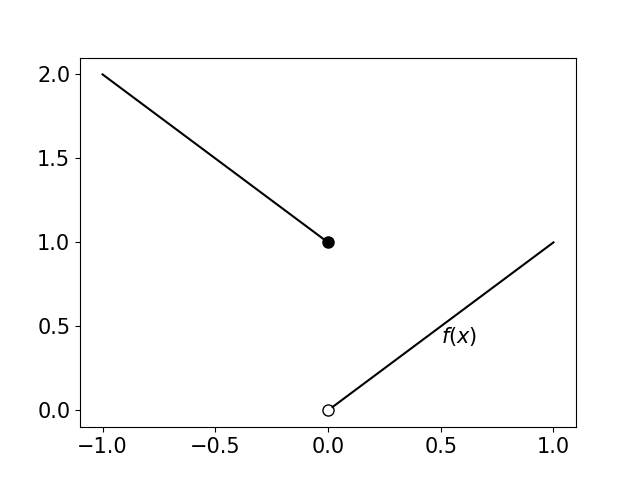
\includegraphics[width=0.4\textwidth]{figures/discontinuous_function.png}};
        \node at (7,0)
        {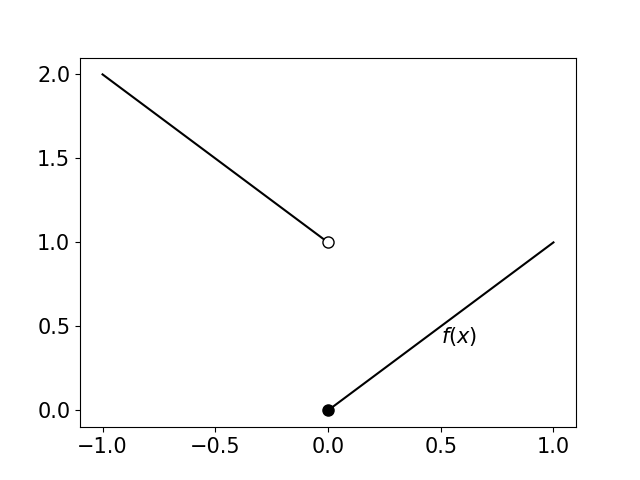
\includegraphics[width=0.4\textwidth]{figures/lsc_function.png}};
        \node at (0,-3) {Minimum tidak tercapai};
        \node at (7,-3) {Minimum tercapai};
    \end{tikzpicture}
    \caption{Kegagalan semikontinuitas bawah dapat menyebabkan infimum tidak
    tercapai.}
    \label{prelim:fig:lsc}
\end{figure}

\noindent\textbf{Deskripsi gambar.} Kedua panel menampilkan fungsi sepotong-sepotong
yang mempunyai lompatan di $x=0$. Pada panel kiri, cabang kanan mendekati titik
kosong $(0,0)$ sementara nilai fungsi di $x=0$ adalah titik penuh $(0,1)$;
infimum $0$ tidak tercapai. Pada panel kanan, titik $(0,0)$ diisi dan titik
$(0,1)$ dibiarkan kosong, sehingga nilai minimum $0$ tercapai.

% H01-S008 | sumber authority/habring/source-v1/preliminaries.tex baris 496--530
% segment-id: d90.hab.v1.ch01.seg0008
\begin{defn}[Koersif]
    Fungsi $f:V\rightarrow(-\infty,+\infty]$ disebut koersif jika
    \begin{equation}
        \lim_{\|x\|\rightarrow\infty}f(x)=\infty.
    \end{equation}
\end{defn}

\begin{theorem}\label{preliminaries:thm:direct_method}
    Misalkan $V$ berdimensi hingga dan
    $f:V\rightarrow(-\infty,\infty]$ proper, koersif, serta semikontinu bawah.
    Maka $f$ mencapai minimumnya pada $V$.\footnote{Asumsi dimensi hingga
    menyediakan kekompakan sekuensial yang dipakai bukti ini. Generalisasi ke
    dimensi tak hingga memerlukan hipotesis tambahan, misalnya refleksivitas dan
    semikontinuitas bawah lemah; ketiga asumsi yang ditampilkan saja tidak cukup.}
\end{theorem}

\begin{proof}
    Bukti mengikuti apa yang disebut \emph{metode langsung}.

    \paragraph{Langkah 1: Ambil barisan peminimum.}
    Misalkan $(x_n)_n$ suatu barisan peminimum\footnote{Sebagai latihan:
    mengapa barisan seperti ini selalu ada?}, yaitu
    \begin{equation}
        \lim_n f(x_n)=\inf_{x\in V}f(x).
    \end{equation}

    \paragraph{Langkah 2: Tunjukkan keterbatasan barisan.}
    Karena $f$ koersif, barisan peminimum harus terbatas. Jika tidak, terdapat
    subbarisan $(x_{n(k)})_k$ dengan $\|x_{n(k)}\|\rightarrow\infty$.
    Koersivitas kemudian memberikan
    \begin{equation}
        f(x_{n(k)})\rightarrow\infty,
    \end{equation}
    yang bertentangan dengan
    \begin{equation}
        f(x_{n(k)})\rightarrow\inf f<\infty.
    \end{equation}

    \paragraph{Langkah 3: Gunakan kekompakan untuk mengambil subbarisan
    konvergen.}
    Berdasarkan~\cref{thm:bolzano}, setiap barisan terbatas dalam ruang vektor
    berdimensi hingga mempunyai subbarisan konvergen. Jadi kita dapat mengambil
    subbarisan $(x_{n(k)})_k$ dengan limit
    $\lim_kx_{n(k)}=\hat x$.

    \paragraph{Langkah 4: Simpulkan dengan semikontinuitas bawah.}
    Berdasarkan semikontinuitas bawah $f$,
    \begin{equation}
        f(\hat x)
        \leq\liminf_{k\rightarrow\infty}f(x_{n(k)})
        =\lim_n f(x_n)
        =\inf_x f(x)
        \leq f(\hat x).
    \end{equation}
    Jadi semua ketaksamaan merupakan kesamaan dan $\hat x$ adalah peminim.
\end{proof}
